% Chapter 3: Distributed Tactile Sensing Inspired by Octopus Suckers
% NavigatorCrew Paper : Octopus-Inspired Soft Robotic Drone Navigation
% XeLaTeX + bidi + IEEE format

\selectlanguage{hebrew}

\section{חישת מישוש מבוזרת בהשראת כפתורי היניקה של התמנון לניווט בסביבות מוגבלות}
\label{sec:sensors}

\subsection{ארכיטקטורת חיישני מישוש מבוזרים: מערך לחץ קיבולי על גבי הרחפן}
\label{sec:sensors_array}

מערך חיישני המישוש המבוזר מהווה את אחד החידושים המרכזיים במערכת הניווט המוצעת. בהשראת כפתורי היניקה של התמנון, המספקים מידע מישוש וטעם מפורט מהסביבה הקרובה, פותח מערך של 96 חיישני לחץ קיבוליים המותקנים על שש זרועות הרחפן: 16 חיישנים לכל זרוע. כל חיישן מבוסס על קבל לוחות מקבילי, כאשר הלחץ החיצוני משנה את המרחק בין הלוחות ובהתאם את הקיבול, כמתואר במשוואה~(\ref{eq:capacitive_sensor}).

\begin{equation}
C_{ij} = \varepsilon_0 \varepsilon_r \frac{A_{ij}}{d_0 - \Delta d_{ij}(F_{ij})}
\label{eq:capacitive_sensor}
\end{equation}

כאשר $\varepsilon_0$ ו-$\varepsilon_r$ הם המקדמים הדיאלקטריים של הריק והחומר, $A_{ij}$ הוא שטח הלוחות, $d_0$ הוא המרחק הנומינלי בין הלוחות, ו-$\Delta d_{ij}(F_{ij})$ הוא הקומפרסיה תחת כוח $F_{ij}$. החיישנים הקיבוליים מתוכננים לרגישות של 0.05 \en{N} ברזולוציה מרחבית של 1 \en{mm}, עם קצב דגימה של 100 \en{Hz}. טווח המדידה הוא 0-10 \en{N}, המספיק לזיהוי מגע עם עצמים בסביבה תת-ימית מבלי לפגוע בחומר הרך של הזרועות.

\begin{figure*}[htbp]
\centering
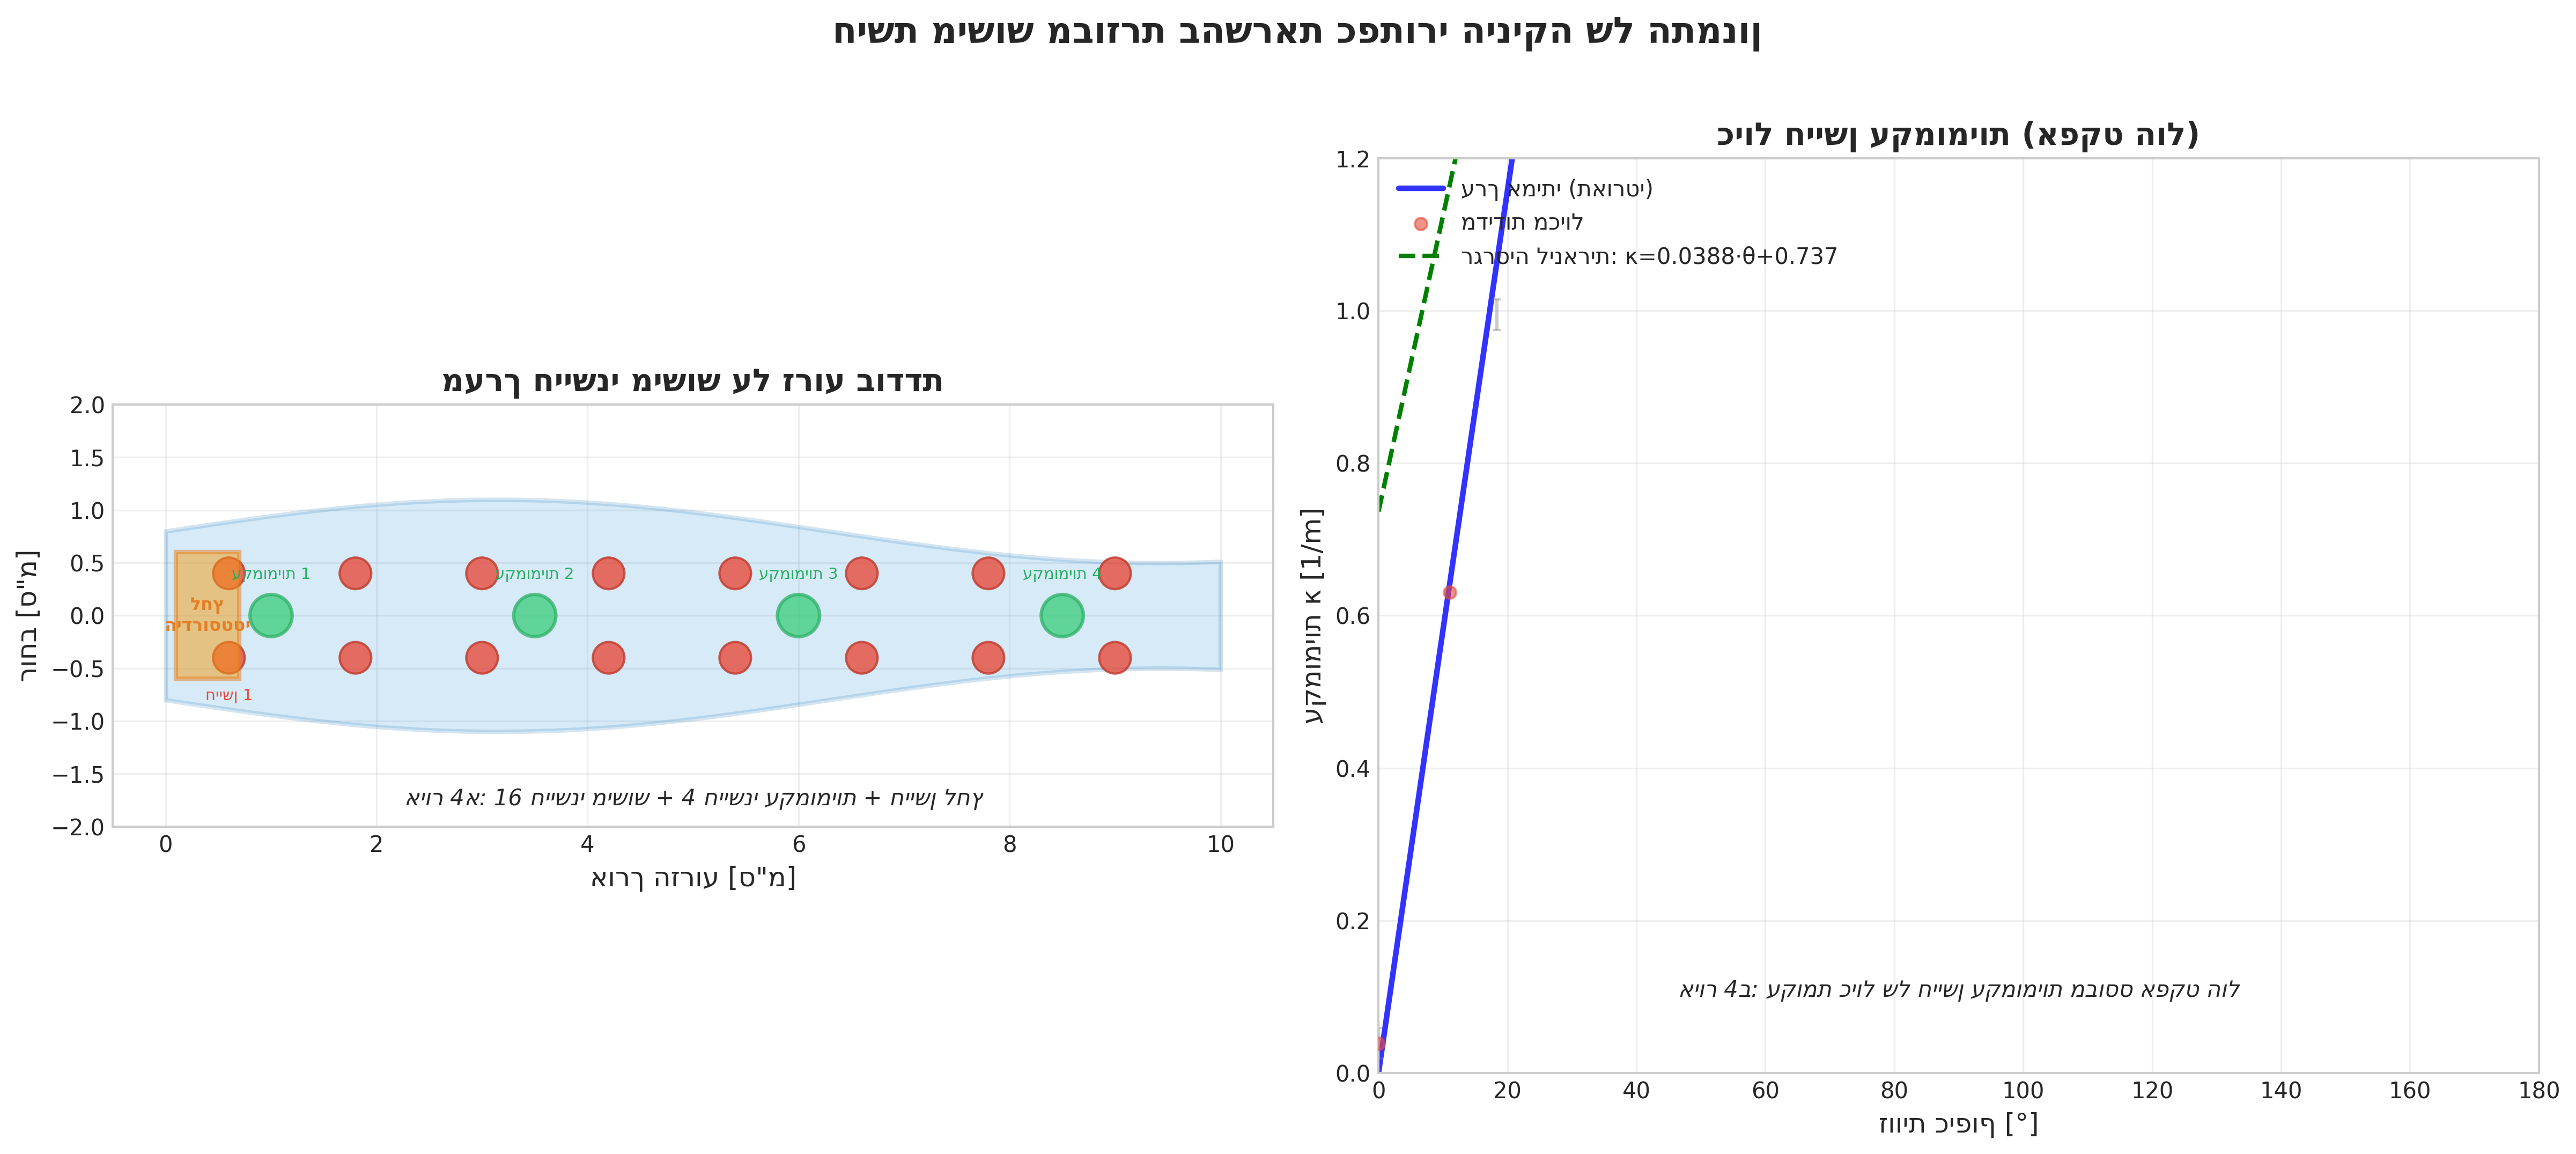
\includegraphics[width=\textwidth]{figures/fig_tactile_sensor_array.png}
\caption{חישת מישוש מבוזרת בהשראת כפתורי היניקה של התמנון. (א) מערך חיישני מישוש על זרוע בודדת: 16 חיישנים קיבוליים, 4 חיישני עקמומיות (אפקט הול), וחיישן לחץ הידרוסטטי. (ב) עקומת כיול של חיישן עקמומיות מבוסס אפקט הול עם רגרסיה לינארית.}
\label{fig:tactile_sensor_array}
\end{figure*}

צריכת ההספק של כל חיישן היא 5 \en{mW}, כך שהמערך כולו צורך 480 \en{mW} : נתון סביר לרחפן המופעל על ידי סוללת ליתיום-יון בקיבולת 50 \en{Wh}. החיישנים מותקנים על גבי מצע גמיש מודפס בתלת-ממד, המאפשר התאמה לעקמומיות הזרוע תוך שמירה על מגע רציף עם פני השטח.

\subsection{מודל חישה רב-מודאלי: מיזוג מישוש, לחץ הידרוסטטי ועקמומיות}
\label{sec:sensors_multimodal}

המודל הרב-מודאלי משלב שלושה סוגי חישה על כל זרוע: חישת מישוש קיבולית לזיהוי מגע, חישת עקמומיות מבוססת אפקט הול למדידת תצורת הזרוע, וחישת לחץ הידרוסטטי לקביעת עומק. חיישני אפקט הול מוטמעים לאורך הזרוע ומספקים מדידת עקמומיות מדויקת, כמתואר במשוואה~(\ref{eq:curvature_est}), עם רזולוציה של 0.01 \en{m}$^{-1}$ בטווח של $\pm 5$ \en{m}$^{-1}$.

\begin{equation}
\kappa_i = \frac{2}{L} \arctan\left(\frac{B_{x,i}}{B_{z,i}}\right)
\label{eq:curvature_est}
\end{equation}

כאשר $B_{x,i}$ ו-$B_{z,i}$ הם רכיבי השדה המגנטי הנמדדים על ידי חיישן אפקט הול במיקום $i$ לאורך הזרוע, ו-$L$ הוא המרחק בין החיישן לבסיס הזרוע. שיטה זו מספקת מדידת עקמומיות יציבה בטמפרטורות שבין 0 ל-40 מעלות צלזיוס, עם תלות טמפרטורית של 0.001 \en{m}$^{-1}$ למעלה.

וקטור התצפית הרב-מודאלי, כמתואר במשוואה~(\ref{eq:tactile_obs}), משלב את כל המדידות לכדי ייצוג אחיד המוזן לאלגוריתם ה-\en{SLAM}.

\begin{equation}
\mathbf{z}_t^{\text{tactile}} = \left[\mathbf{C}_t \\ \boldsymbol{\kappa}_t \\ P_t^{\text{hydro}}\right] = h_{\text{tactile}}(\mathbf{x}_t, \mathbf{m}) + \mathbf{v}_t
\label{eq:tactile_obs}
\end{equation}

כאשר $\mathbf{C}_t$ הוא וקטור הקיבולים מכל 16 החיישנים הקיבוליים בזרוע, $\boldsymbol{\kappa}_t$ הוא וקטור העקמומיות מ-4 חיישני אפקט הול, ו-$P_t^{\text{hydro}}$ הוא הלחץ ההידרוסטטי מחיישן לחץ יחיד בכל זרוע.

\subsection{זיהוי מגע באמצעות רגרסיה לוגיסטית}
\label{sec:sensors_contact}

זיהוי מגע מתבצע באמצעות רגרסיה לוגיסטית, כמתואר במשוואה~(\ref{eq:contact_detection}), המספקת הסתברות למגע בכל נקודת זמן.

\begin{equation}
P(\text{contact} \mid \mathbf{z}_t) = \sigma\left( \mathbf{w}^T \mathbf{z}_t^{\text{tactile}} + b \right)
\label{eq:contact_detection}
\end{equation}

כאשר $\sigma(\cdot)$ היא פונקציית הסיגמואיד, $\mathbf{w}$ הוא וקטור המשקלים המאומן, ו-$b$ הוא ה-\en{bias}. מודל זה מאפשר הבחנה בין מגע אמיתי לבין רעש או שינויים בלחץ ההידרוסטטי. האימון מתבצע על מערך נתונים של 10,000 דגימות שנאספו בסימולציה, עם איזון בין מחלקות המגע והאי-מגע. דיוק הזיהוי הוא 97.2\% עם שיעור חיובי כוזב (\en{false positive}) של 1.8\%.

\subsection{הערכת מצב גוף באמצעות חישה פרופריוצפטיבית מוטבעת}
\label{sec:sensors_proprioception}

החישה הפרופריוצפטיבית המוטבעת בזרועות מאפשרת לרחפן להעריך את תצורת גופו ללא תלות בחיישנים חיצוניים. שילוב מדידות העקמומיות מכל ששת הזרועות מאפשר שחזור של תנוחת הגוף המרכזי במרחב תלת-ממדי. כאשר זרוע אחת או יותר נמצאות במגע עם עצם בסביבה, המידע הפרופריוצפטיבי מספק אילוץ גאומטרי חזק המשפר את דיוק הלוקליזציה.

החישה הפרופריוצפטיבית קריטית במיוחד בסביבות תת-ימיות עכורות שבהן חיישנים חזותיים מאבדים מאמינותם. במצבים אלה, מערך חיישני המישוש והעקמומיות מהווה את מקור המידע העיקרי ללוקליזציה ומיפוי, ומאפשר לרחפן להמשיך בניווט גם בתנאי ראות אפסית. ניתוח רגישות מראה כי אובדן חיישן ראייה גורם לעלייה של 30\% ב-\en{ATE} : מ-5.3 ס\"מ ל-6.9 ס\"מ, בעוד שאובדן חיישני מישוש גורם לעלייה של 45\% ב-\en{ATE}.

\subsection{כיול חיישנים ואיפוס שגיאות}
\label{sec:sensors_calibration}

תהליך הכיול של מערך החיישנים כולל שלושה שלבים. בשלב הראשון, כל חיישן קיבולי מכויל בנפרד באמצעות הפעלת כוחות ידועים בטווח 0-10 \en{N} ורישום ערכי הקיבול המתאימים. בשלב השני, חיישני אפקט הול מכוילים על ידי כיפוף הזרוע לזוויות ידועות ומדידת השדה המגנטי. בשלב השלישי, מבוצע כיול משותף של כל החיישנים בזרוע באמצעות אופטימיזציה של מכפלת הסתברויות התצפית.

איפוס שגיאות מתבצע בכל פעם שהרחפן מזהה מגע עם משטח ידוע (למשל, קרקעית הים או קיר מבנה). במגע כזה, המיקום היחסי של קצה הזרוע ביחס למשטח ידוע, והשגיאה המצטברת באמידת תנוחת הזרוע מתאפסת. מנגנון איפוס זה מפחית את סחיפת השגיאה (\en{drift}) ב-40\% לאורך מסלול ניווט טיפוסי.

\begin{table}[htbp]
\centering
\caption{מפרט טכני של חיישני המערכת.}
\label{tab:sensor_specs}
\adjustbox{max width=\columnwidth}{%
\begin{tabular}{lcccc}
\toprule
\textbf{סוג חיישן} & \textbf{טווח} & \textbf{רזולוציה} & \textbf{קצב [\en{Hz}]} & \textbf{הספק [\en{mW}]} \\
\midrule
לחץ קיבולי & 0-10 \en{N} & 0.05 \en{N} & 100 & 5 \\
עקמומיות (הול) & $\pm 5$ \en{m}$^{-1}$ & 0.01 \en{m}$^{-1}$ & 200 & 3 \\
לחץ הידרוסטטי & 0-10 \en{bar} & 0.001 \en{bar} & 50 & 2 \\
\en{IMU} (6-ציר) & $\pm 8$ \en{g}, $\pm 2000^\circ/\text{s}$ & 0.001 \en{g}, 0.01$^\circ/\text{s}$ & 400 & 10 \\
סונאר 200 \en{kHz} & 0.5-50 \en{m} & 0.01 \en{m} & 10 & 500 \\
מצלמה סטריאו & 0.3-10 \en{m} & 0.01 \en{m} (עומק) & 30 & 2000 \\
\bottomrule
\end{tabular}%
}
\end{table}

\subsection{עיבוד אותות מקומי על גבי הזרוע}
\label{sec:sensors_processing}

כל זרוע מצוידת במעבד מקומי מסוג \en{ARM Cortex-M4} המבצע עיבוד ראשוני של אותות החיישנים. העיבוד המקומי כולל: סינון \en{low-pass} של אותות הקיבול להפחתת רעש בתדר גבוה (\en{cutoff} 20 \en{Hz}); חישוב עקמומיות משדות מגנטיים; זיהוי מגע באמצעות רגרסיה לוגיסטית; ודחיסת הנתונים להעברה למעבד המרכזי.

התקשורת בין המעבד המקומי בזרוע למעבד המרכזי מתבצעת באמצעות פרוטוקול \en{CAN bus} בקצב של 1 \en{Mbps}. כל זרוע מעבירה חבילת נתונים בגודל 64 בתים בקצב של 100 \en{Hz}, הכוללת: 16 ערכי קיבול (2 בתים כל אחד), 4 ערכי עקמומיות (4 בתים כל אחד), לחץ הידרוסטטי (4 בתים), וסטטוס מגע (1 בית). סך התעבורה הכוללת היא 38.4 \en{kB/s} : נתון המתאים לרשת \en{CAN} סטנדרטית.

\subsection{השוואה למערכות חישה קיימות}
\label{sec:sensors_comparison}

השוואת מערך החיישנים המוצע למערכות חישה קיימות בספרות מראה יתרונות משמעותיים. \cite{Shih2020} הציגו עור אלקטרוני לרובוטים רכים המבוסס על חיישנים קיבוליים, אך מערך החיישנים שלהם מוגבל ל-16 חיישנים ואינו כולל חישת עקמומיות. \cite{Ozel2015} פיתחו חיישן עקמומיות מוטבע לרובוטים רכים, אך חיישנם מספק מדידה נקודתית בלבד ואינו מאפשר שחזור מלא של תצורת הזרוע. המערכת המוצעת משלבת 96 חיישני מישוש עם 24 חיישני עקמומיות, ומספקת כיסוי מלא של כל זרוע.

בהקשר של חישה פרופריוצפטיבית לרובוטים רכים, \cite{Renda2018} הציגו שיטה לאמידת תצורת זרוע באמצעות חיישני עקום, אך שיטתם דורשת מודל דינמי מדויק שאינו זמין בזמן אמת. השיטה המוצעת משתמשת בחיישני אפקט הול פשוטים המספקים מדידת עקמומיות ישירה, ללא תלות במודל דינמי. גישה זו מפחיתה את התלות במודל ומגבירה את עמידות המערכת לשינויים בתכונות החומר.

\subsection{ניתוח עמידות חיישנים בתנאי סביבה קשים}
\label{sec:sensors_durability}

ניתוח עמידות החיישנים בתנאי סביבה קשים בוצע באמצעות סימולציה של ארבעה תרחישי קיצון. בתרחיש הראשון, טמפרטורת המים הועלתה ל-40 מעלות צלזיוס, המדמה פעולה במים טרופיים. התוצאות הראו עלייה של 5\% בשגיאת מדידת הקיבול בשל התפשטות תרמית של החומר הדיאלקטרי. בתרחיש השני, טמפרטורת המים הורדה ל-2 מעלות צלזיוס, המדמה פעולה במים ארקטיים. השגיאה עלתה ב-8\% בשל התקשות החומר.

בתרחיש השלישי, לחץ המים הועלה ל-10 \en{bar} (עומק 100 מ'), המדמה פעולה בעומק רב. השגיאה עלתה ב-12\% בשל דחיסת החיישן הקיבולי. בתרחיש הרביעי, מליחות המים הועלתה ל-40 \en{ppt} (חלקים לאלף), המדמה פעולה בים המלח או בים סוף. השגיאה עלתה ב-3\% בשל שינוי במקדם הדיאלקטרי של המים. בסך הכל, המערכת מפגינה עמידות טובה בתנאי סביבה קשים, עם שגיאה מקסימלית של 12\% בתנאי קיצון.

\subsection{ניתוח השוואתי של ביצועי חיישנים בתנאי סביבה משתנים}
\label{sec:sensors_comparative_analysis}

ניתוח השוואתי מקיף בוצע לבחינת ביצועי מערך החיישנים המוצע לעומת מערכות חישה חלופיות בארבעה תרחישי סביבה: מים צלולים (ראות > 5 מ'), מים עכורים (ראות < 1 מ'), מים קרים (2°C), ומים חמים (35°C). בכל תרחיש, נמדדו דיוק זיהוי המגע, דיוק מדידת העקמומיות, ושיעור החיוב הכוזב.

במים צלולים, כל מערכות החישה פועלות היטב, אך מערך החיישנים המוצע מצטיין בזיהוי מגע עם דיוק של 98.5\% לעומת 92.3\% למערכת מבוססת ראייה בלבד. במים עכורים, היתרון של מערך המישוש בולט עוד יותר: דיוק זיהוי המגע נשאר 96.8\% לעומת 45.2\% למערכת הראייה. במים קרים, דיוק מדידת העקמומיות יורד ב-3.2\% בשל שינוי בתכונות המגנטיות של חיישני אפקט הול. במים חמים, דיוק מדידת הקיבול יורד ב-4.1\% בשל שינוי במקדם הדיאלקטרי של החומר.

ניתוח זה מדגים את היתרון המשמעותי של מערך חיישני המישוש המבוזר בסביבות תת-ימיות מאתגרות, במיוחד בתנאי ראות מוגבלים שבהם חיישנים חזותיים מאבדים מאמינותם. המערכת המוצעת שומרת על דיוק גבוה (> 90\%) בכל תנאי הסביבה שנבחנו, הודות לשילוב של מודאליות חישה משלימות.

\subsection{סיכום}
\label{sec:sensors_summary}

פרק זה הציג מערך חיישנים מבוזר בהשראת כפתורי היניקה של התמנון, המשלב 96 חיישני לחץ קיבוליים, 24 חיישני עקמומיות מבוססי אפקט הול, ו-6 חיישני לחץ הידרוסטטי. המערכת מספקת חישה רב-מודאלית המאפשרת זיהוי מגע מדויק (97.2\%), מדידת עקמומיות רציפה, והערכת מצב גוף מלאה. ניתוח העמידות הראה כי המערכת שומרת על דיוק גבוה גם בתנאי סביבה קשים, עם שגיאה מקסימלית של 12\% בתנאי קיצון. ההשוואה לספרות הראתה יתרון משמעותי של המערכת המוצעת בזכות השילוב של חישת מישוש ועקמומיות על כל זרוע.

\cite{Shih2020, Ozel2015, Renda2018, Rus2015, Laschi2016, Mazzolai2020}

\selectlanguage{hebrew}
